\item Theorem: $n \in \mathbb{N} \wedge n \neq 1 \rightarrow \exists p (p \in \mathbb{P} \wedge p|n)$

But first, Prime or composite lemma: Any natural number $p$ greater than one is either prime or composite. In other words if $p$ is not composite, it is prime. If $p$ is not prime, it is composite.

\textit{Every now and then, I feel I need to prove one thing formally so I don't get to relaxed with my form.}

\begin{proof}
$p$ is not composite & Premise \\
$\neg \exists a, b \in \mathbb{N} (p = ab \wedge 1 < a, b < p) $ & Definition of composite (negated) \\
$\neg \exists a, b \in \mathbb{N} (p = ab \wedge 1 < a < p) $ & Simplification \\
$\forall a, b \in \mathbb{N} \neg(p = ab \wedge 1 < a < p) $ & Quantifier exchange \\
$\neg (p = ab \wedge 1 < a < p) $ & Universal instantiation \\
$\neg (p = ab) \wedge \neg (1 < a < p) $ & DeMorgan's law \\
$p = ab \rightarrow \neg (1 < a < p) $ & Conditional disjunction \\
$p = ab \rightarrow \neg 1 < a \wedge a < p $ & Property of inequality \\
$p = ab \rightarrow \neg (1 < a) \vee \neg (a < p) $ & DeMorgan's law \\
$p = ab \rightarrow 1 \geq a \vee a \geq p $ & Property of inequality \\
$p = ab \rightarrow (1 = a \wedge a \geq p) $ & Property of Natural numbers \\
$p = ab \rightarrow (1 = a \wedge a = p) $ & $a|p \rightarrow a \leq p$ \\
$a|p \rightarrow (1 = a \wedge a = p) $ & Definition of division \\
$\forall a (a|p \rightarrow (1 = a \vee a = p))$ & Universal generalization \\
$p$ is prime & Definition of primes
\end{proof}

\begin{proof}
$p \in \mathbb{P}$ & Premise \\
$\neg (\forall d (d|n \rightarrow (d = 1 \vee d = n)))$ & Definition of prime \\
$\exists d \neg (d|n \rightarrow (d = 1 \vee d = n))$ & Quantifier exchange \\
$\exists d \neg (\neg(d|n) \vee (d = 1 \vee d = n))$ & Conditional disjunction \\
$\exists d \neg \neg (d|n) \wedge \neg (d = 1 \vee d = n)$ & DeMorgan's law \\
$\exists d d|n \wedge \neg (d = 1 \vee d = n)$ & Double Negation \\
$\exists d d|n \wedge \neg d = 1 \wedge \neg d = n$ & DeMorgan's law \\
$\exists d d|n \wedge 1 < d < n$ & Inequality over naturals \\
$\exists d \exists c (cd = n) \wedge 1 < d < n$ & Definition of divides \\
$\exists d \exists c (cd = n \wedge 1 < c < n) \wedge 1 < d < n$ & Inequality over naturals \\
$p$ is composite
\end{proof}

Because of this, let $a \notin \mathbb{P}$ stand for `$a$ is composite' (only when $a \neq 1$).

Transitivity of divisibility Lemma: $a|b \wedge b|c \rightarrow a|c$

\begin{proof}
$an = b$ & Definition of divides \\
$bm = c$ & Definition of divides \\
$anm = c$ & Substitution \\
$a|c$ & Definition of divides
\end{proof}

Theorem: $n \in \mathbb{N} \wedge n \neq 1 \rightarrow \exists p (p \in \mathbb{P} \wedge p|n)$

\begin{proof}
If $p \in \mathbb{P}$ & \\
$p = 1p$ & Identity of Multiplication \\
$p|p$ & Definition of divides $\square$ \\
Otherwise, $p \notin \mathbb{P}$ \\
Follow this algorithm: \\
$p = a_1 b_1 \wedge 1 < a_1, b_1 < p \fs a_1, b_1$ & Definition of composite ($\notin \mathbb{P}$) \\
$a_1|p$ & Definition of divides \\
If $a_1 \in \mathbb{P}$ halt \\
Otherwise $a_1 \notin \mathbb{P}$ \\
$a_1 = a_2 b_2 \wedge 1 < a_2 < a_1 < p$ & Definition of composite \\
\vdots \\
$a_i = a_{i+1} b_{i+2} \wedge 1 < a_i < a_{i-1} < \underbrace{\dots}_{i \mathrm{~times}} < p$ & Definition of composite \\
$a_{i+1}|a_{i}$ & Definition of divides \\
If $a_i \in \mathbb{P}$ halt \\
Otherwise $a_i \notin \mathbb{P}$ and repeat \\
\vdots \\
$a_{n - 1} = a_n b_n \wedge 1 < a_n < \underbrace{\dots}_{p \mathrm{~times}} < p$ \\
There can not be $p$ unique numbers between $1$ and $p$\\
Therefore this process must terminate (call that place $a_j$) & Algorithm halts\\
$a_j \in \mathbb{P} \wedge a_j|a_{j-1} \wedge a_{j-1}|a_{j-2} \wedge \dots \wedge a_1|p$ & Condition for termination \\
$a_j \in \mathbb{P} \wedge a_j|p$ & Transitivity of divisibility lemma
\end{proof}

\item $\{2, 3, 5, 7, 11, 13, 17, 19, 23, 29, 31, 37, 41, 43, 47, 51, 53, 59, 61, 67, 71, 73, 79, 83, 89, 97\}$

\item Theorem: $n \in \mathbb{P} \leftrightarrow \neg \exists p (p \in \mathbb{P} \wedge 1 < p \leq \sqrt{n} \wedge p|n)$

I will simply prove the biconditional with both sides negated.

Theorem equivalent: $n \notin \mathbb{P} \leftrightarrow \exists p (p \in \mathbb{P} \wedge 1 < p \leq \sqrt{n} \wedge p|n)$

\begin{proof}
$\rightarrow$ \\
$n \notin \mathbb{P}$ & Premise \\
$ab = n \fs 1 < a, b < n$ & Definition of $\notin \mathbb{P}$ \\
Assume the following for contradiction \\
$a > \sqrt{n}$ & Assume \\
$b > \sqrt{n}$ & Assume\\
$n > 1$ & Premise \\
$\sqrt{n} > 1$ & Property of square root \\
$a > \sqrt{n} > 1$ & \\
$b > \sqrt{n} > 1$ & Property of inequality\\
$ab > n$ & Property of inequality \\ & (since they are all greater than 1) \\
$ab = n$ & Definition of $a$ and $b$ \\
$\neg (a > \sqrt{n}) \vee \neg (b > \sqrt{n})$ & Contradiction \\
$a \leq \sqrt{n} \vee b \leq \sqrt{n}$ & Property of inequality \\
Either way: \\
$\exists p (1 < p \leq \sqrt{n} \in \mathbb{N})$ & Existential instantiation\\ &(on $a$ or on $b$)
\end{proof}

\begin{proof}
$\leftarrow$ \\
$p \in \mathbb{P} \wedge 1 < p \leq \sqrt{n} \wedge p|n$ & Universal instantiation \\
$\sqrt{n} < n$ & Property of positive numbers \\
$1 < p < n$ & Property of inequalities \\
$\exists c (1 < c < n \wedge pc = n)$ & Definition of divides \\
$1 < p, c < n \wedge pc = n$ & Restatement \\
$n \notin \mathbb{P}$ & Definition of composite
\end{proof}

\item 
$101 < 121$ \\
$\sqrt{101} < \sqrt{121}$ since they are all positive \\
$\sqrt{101} < 11$ \\
$\{p | p \in \mathbb{P} \wedge p < 11\} = \{2, 3, 5, 7\}$ \\
$2 \not | 101 \wedge 3 \not | 101 \wedge 5 \not | 101 \wedge 7 \not | 101$ \\
$\therefore 101 \in \mathbb{P}$

\item 
\newcommand*\circled[1]{
\tikz[baseline=(char.base)]{
\node[shape=circle,draw,inner sep=1pt] (char) {#1};
}
}

\begin{python}[tools.py]
output = r'$\{$'
for x in range(2, 101):
    if is_prime(x):
        output += r'$\circled{{{x}}}$, '.format(**locals())
    else:
        output += r'$\cancel{{{x}}}$, '.format(**locals())
output = output[:-2]
output += r'$\}$'
print output
\end{python}

\item 
The blue line is $\frac{\Pi(x)}{x}$.

The green line is $\frac{1}{\ln(x)}$

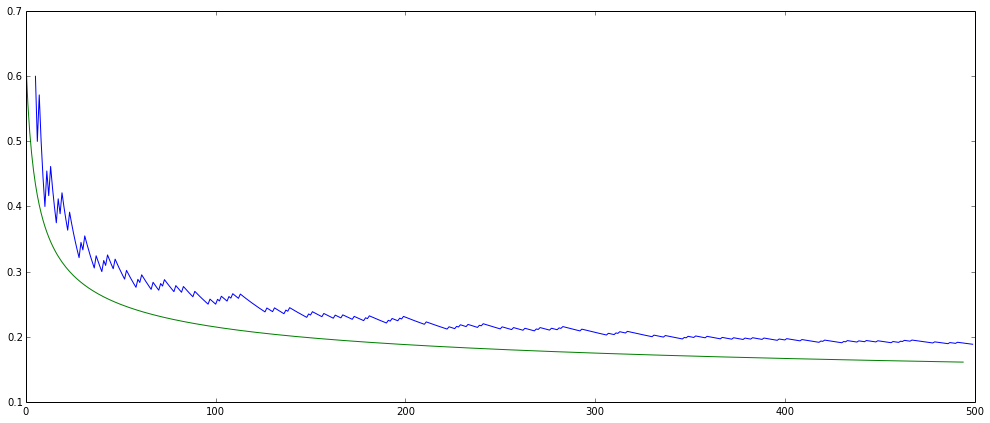
\includegraphics[width=5.5in]{primes_small.png}

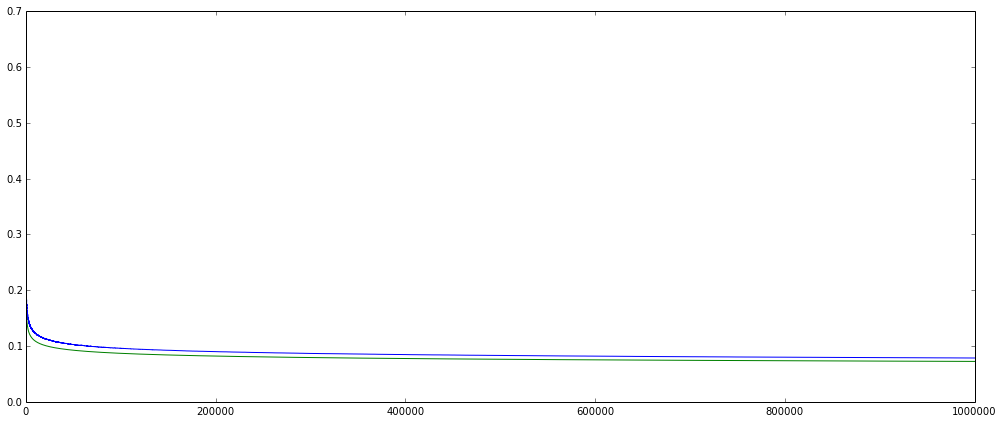
\includegraphics[width=5.5in]{primes_large.png}

\item Every natural number excluding one has a prime factorization.

$\forall_{n \in \mathbb{N}\backslash\{1\}} (\exists _{\{p_1, p_2, \dots, p_n\} \subset \mathbb{P}} ~ \exists _{\{r_1, r_2, \dots r_3\} \subset \mathbb{N}} (\prod\limits^i p_i^{r_i} = n))$

\item 

Coprime primes lemma: any prime number ($p$) is coprime to any other prime number ($q$).

\begin{proof}
$(p, q)|p \wedge (p, q)|q $ & Definition of GCD \\
$(a = 1 \vee a = q) \wedge (a = 1 \vee a = p)$ & Definition of prime \\
$p \neq q$ & Premise \\
$a = 1 \vee a = p = q$ & Simplification \\
$a = 1$ & Disjunctive syllogism
\end{proof}

\begin{proof}
$p \neq | 1$ & Premise \\
$p|(\prod\limits_{i=1}^{n} q_i)$ & Definition of divides \\
$\forall i \{ q_i \neq p\}$ & Assume for contradiction \\
$\forall i \{ (q_i, p) = 1\}$ & Coprime primes lemma (applied over all $p_i$) \\
$p | q_1 \prod\limits_{i = 2}^n q_i$ & Algebra \\
$(p, q_1) = 1$ & Coprime primes lemma \\
$p|\prod\limits_{i=2}^n q_i$ & Theorem 1.41 (Base case) \\
$p|\prod\limits_{i=j}^n q_i$ & Assume (Inductive hypothesis) \\
$p|q_{j+1} \prod\limits_{i=j+1}^n q_j$ & Algebra \\
$(p, q_j) = 1$ & Coprime primes lemma \\
$p|\prod\limits_{i=j+1}^n$ & Theorem 1.41 (Inductive Step)\\
$p|\prod\limits_{i=n}^n$ & Inductive axiom \\
$p|1 \wedge p \neg | 1$ & Product rule \\
$\neg \forall i \{ q_i \neq p\}$ Contradiction \\
$\exists i\{ q_i = p\}$ & Simplification
\end{proof}

\item Every natural number excluding one has a \textbf{unique} prime factorization.

$\forall_{n \in \mathbb{N}\backslash\{1\}}
(\exists _{\{p_1, p_2, \dots, p_n\} \subset \mathbb{P}} ~
\exists _{\{r_1, r_2, \dots, r_n\} \subset \mathbb{N}}
\exists _{\{q_1, q_2, \dots, q_m\} \subset \mathbb{P}} ~
\exists _{\{t_1, t_2, \dots, t_m\} \subset \mathbb{N}}
(\prod\limits^i p_i^{r_i} = \prod\limits^j q_j^{t_j}) \rightarrow
m = n \wedge \{p_1, p_2, \dots, p_n\} = \{q_1, q_2, \dots, q_m\} \wedge (p_i = q_j \rightarrow r_i = t_j))$

\item $
\begin{array}[t]{rl}
12!& = 2 \cdot 3 \cdot 4 \cdot 5 \cdot 6 \cdot 7 \cdot 8 \cdot 9 \cdot 10 \cdot 11 \cdot 12 \\
&= 2 \cdot 3 \cdot 2^2 \cdot 5 \cdot (2 \cdot 3) \cdot 7 \cdot 2^3 \cdot 3^2 \cdot (2 \cdot 5) \cdot 11 \cdot (2^2 \cdot 3) \\
&= 2^{10} \cdot 3^5 \cdot 5^2 \cdot 7 \cdot 11 \\
\end{array}
$

\item $25! = 1 \cdot 2 \cdot 3 \dots 25$ \\
%5 multiples of 5 were written down \\
%1 multiple of 25 was written down \\
The largest power of 5 that divides 25 is $5^{5 + 1}$ \\
%12 multiples of 2 were written down \\
%5 multiples multiples of 4 were written down \\
%3 multiples of 8 were written down \\
%1 multiple of 16 was written down \\
The largest power of 2 that divides 25 is $2^{12+5+3+1}$ \\
$5^{5 + 1} \cdot 2^{12+5+3+1} | 25$ \\
$5^{6} \cdot 2^{21} | 25$ \\
$10^{6} \cdot 2^{21 - 6} | 25$ \\
The largest power of 10 that divides 25 is $10^6$ \\
There are 6 zeros at the end of $25!$

\newcommand{\pf}{\mathrm{pf}}
\item \(a|b \leftrightarrow \pf(a) \subseteq \pf(b)\)
\begin{proof}
\(a|b\) & Premise \\
\(ma = b \fs m \in \mathbb{Z}\) & Definition of divides \\
\(\pf(ma) = \pf(b) \fs m \in \mathbb{Z}\) & \(\pf\) is injective \\
\(\pf(m) + \pf(a) = \pf(b) \) & \(\pf\) of product theorem \\
\( \pf(a) \subseteq \pf(b)\) & addend-subset theorem 
\end{proof}

\item \(a^2 | b^2 \leftrightarrow a | b\)
\begin{proof}
\(a^2 | b^2\) & Premise \\
\(a = p_1^{r_1} p_2^{r_2} \dots\) \\ 
\(b = q_1^{t_1} q_2^{t_2} \dots\) & Fundamental Theorem of Rithmetic \\
\(a^2 = p_1^{2r_1} p_2^{2r_2} \dots\) \\
\(b^2 = q_1^{2t_1} q_2^{2t_2} \dots\) & Algebra \\
\(\pf(a) \subset \pf(b)\) & I don't know \\
\end{proof}

\item \(\gcd(3^14 \cdot 7^22 \cdot 11^5 \cdot 17^3, 5^2 \cdot 11^4 \cdot 13^8 \cdot 17) = 11^4 \cdot 17\)

\item \(\lcm (3^14 \cdot 7^22 \cdot 11^5 \cdot 17^3, 5^2 \cdot 11^4 \cdot 13^8 \cdot 17) = 3^14 \cdot 5^2 \cdot 7^22 \cdot 11 \cdot 13^8 \cdot 17^2 \cdot 11^4 \cdot 17\)

\item \(\gcd(a, b) = \pf(a) \cap \pf(b)\)

\(\lcm(a, b) = \pf(a) \cup \pf(b)\)

\item It depends on how easy it is to factor. I easily recognize the prime factorization if and only if the prime factorization method is clearly better.

In general, factoring a number assuming the density of primes is proportional \(\frac{1}{\ln(x)}\) as proposed in 2.6, the number of primes less than \(n\) should be \(\int \limits_{x=1}^{x=n} \frac{1}{\ln(x)} \, dx = n \ln(n) - n - 1 \). Lets assume I need to do long division to test for divisibility. Long division has complexity of \(\mathcal{O}(log(x))\). Now for every prime, I need to do this check. The worst case scenario is that the number under test is itself prime, therefore the problem does not reduce as I continue (what normally happens when factoring). The worst-case run-time is \(\mathcal{O}(log^2(n)\) where \(n\) is the number under test.

On the other hand, the Euclidean Algorithm replaces the larger number with the difference of the two. For the worst-case scenario, we will assume the difference is such that half the next term is close to half of the smaller term. Thus we divide by two every time. The worst-case run-time is \(\mathcal{O}(log(n)\).

Because of this, I think the Euclidean Algorithm is more efficient as the $n$ approaches $\infty$.

\item 

\begin{tabular}{l}
If \(n = 1\), the theorem is true, \\
since there is only one number to pick from (\textbf{Base Case}) \\
The theorem holds for picking \(n\) numbers less than or equal to \(\{1, \dots 2n\}\) (\textbf{Inductive Hypothesis}) \\
Lets say we pick \(n + 1\) numbers less than or equal to \(2(n + 1)\) \\
We pick from \(1 to 2n + 2\) \\
We pick from \(\{1, \dots, 2n, 2n + 1, 2n + 2\}\) \\
There are three options: \\
First, we can pick \(n + 1\) numbers from \(\{1, \dots, 2n\) \\
Second, we can pick \(n\) numbers from \(\{1, \dots, 2n\}\) and \(1\) number from \(\{2n+1, 2n+2\}\) \\
Third, we can pick \(n - 1\) numbers from \(\{1, \dots, 2n\}\) and both \(\{2n + 1, 2n + 2\}\) \\
In the first case, the theorem holds, by the Inductive Hypothesis \\
In the second case, the theorem holds by the Inductive Hypothesis \\
In the third case, the 
\end{tabular}

\setcounter{enumii}{23}

\item Let $n \in \mathbb{Q}$ and $x \in\mathbb{N}$. $x^n \in \mathbb{N} \vee x^n \notin \mathbb{Q}$

\setcounter{enumii}{27}

\item $(b, c) = 1 \rightarrow (a, bc) = (a, b) \cdot (a, c)$

\begin{proof}
$a = \prod A$ where $A \subset \mathbb{P}$ \\
$b = \prod B$ where $B \subset \mathbb{P}$ \\
$c = \prod C$ where $C \subset \mathbb{P}$ & Fundamental theorem \\
$$
$B \cap C = \emptyset$ & 
\end{proof}

%%% Local Variables:
%%% mode: latex
%%% TeX-master: "main"
%%% End:
